% \documentclass{article}

% % Figure setup
% \usepackage{graphicx}
% \graphicspath{{./images/}}
% \usepackage{subcaption}

% % Ref setup
% \usepackage{hyperref}

% % Cite setup
% \usepackage{cite}

% % Font setup
% \usepackage{fontspec}
% \setmainfont{Times New Roman}

% % Lang setup
% \usepackage{polyglossia}
% \setdefaultlanguage{russian}
% \setotherlanguage{english}

% \renewcommand{\UrlFont}{\ttfamilylatin}

\chapter{Исследование фазовых переходов, магнитных, термодинамических и критических свойств в магнитных спиновых системах}
% \author{Магомедов Магомед Алиевич}
% \date{}

% \begin{document}

% \maketitle

%% \begin{abstract}
%    Методом Ванга-Ландау исследована векторная пятихвершинная модель Поттса на треугольной решетке с учетом конкурирующего обменного взаимодействия между первыми и вторыми ближайшими соседями. Вычислена плотность состояний системы $g(E)$, определены магнитные структуры основного состояния и рассчитаны температурные зависимости различных термодинамических параметров, таких как внутренняя энергия $E$, теплоемкость $C$, энтропия $S$. Показано, что в зависимости от знака обменного взаимодействия между спинами, основное состояние может быть ферромагнитным либо сильно вырожденным.
%% \end{abstract}
%
%\textbf{Целью настоящей работы} является исследование векторной модели Поттса с числом состояний $q=5$ на треугольной решетке методами вычислительной физики.
%
%\textbf{Объектом исследования} являлась векторная модель Поттса с числом состояний $q=5$ на треугольной решетке.
%
%\textbf{Методы исследования.} Для исследования векторной модели Поттса с числом состояний $q=5$ на треугольной решетке нами был разработан комплекс программ для ЭВМ, основанный на алгоритме Ванга-Ландау. Методика исследований, предложенная нами, позволяет не только рассчитать температурные зависимости различных термодинамических параметров, но также определить структуру основного состояния системы, выявить наличие фрустрации или вырождения основного состояния, а также рассчитать энтропию и свободную энергию, что невозможно при использовании других методов. Важной особенностью реализованного нами метода является возможность снятия <<снимка>> основного состояния -- сохранения в графическом файле структуры основного состояния, которая позволяет рассмотреть, какое упорядочение реализуется в системе вблизи абсолютного нуля.

\section{Введение}

Исследование фазовых переходов (ФП), магнитных, термодинамических и критических свойств в магнитных спиновых системах представляет большой теоретический и экспериментальный интерес. Это связано с тем, что для большинства реальных магнитных спиновых систем характерны возмущения различной природы, такие как анизотропия, взаимодействия следующих за ближайшими соседей, внешнее магнитное поле, тепловые и квантовые флуктуации, немагнитные примеси, дефекты, деформации и др. Присутствие этих факторов может повлиять на природу ФП и термодинамические характеристики таких систем \cite{bib:mma-1,bib:mma-2,bib:mma-3,bib:mma-4,bib:mma-5,bib:mma-6,bib:mma-7,bib:mma-8,bib:mma-9,bib:mma-10,bib:mma-11}. Для изучения особенностей термодинамического поведения и природы ФП успешно используются различные решеточные модели. На их основе получено большое количество интересных результатов. Решеточные спиновые модели позволяют описать целый ряд реальных магнитных материалов.

Одной из моделей, применяемых для описания физических систем, является векторная модель Поттса с числом состояний спина $q$. Нами в данном исследовании рассматривается векторная модель Поттса с числом состояний спина $q=5$ на треугольной решетке. Магнитные материалы на треугольной решетке представляют особый интерес для исследователей. Антиферромагнетики на треугольной решетке представляют собой геометрически фрустрированные спиновые системы, которые исследуются уже давно. Для фрустрированных систем существует совсем немного надежно установленных фактов. Большинство имеющихся результатов получены для модели Изинга, Гейзенберга и Поттса с числом состояний спина $q = 2$, $3$ и $4$.

Многие физические свойства часовой модели зависят от значения $q$. В случае, когда $q = 2$, $3$, $4$, эта модель имеет точное решение. Векторная модель Поттса сводится к модели Изинга и $Z_3$ модели Поттса при $q = 2$ и $3$, соответственно. При $q = 4$ данная модель эквивалентна двум копиям модели Изинга. Установлено, что для этих трех случаев в системе наблюдается ФП второго рода из высокотемпературной парамагнитной фазы в низкотемпературную ферромагнитную упорядоченную фазу. Когда $q \to \infty$ данная векторная модель Поттса сводится к стандартной $XY$ модели. В этом случае спонтанного нарушения симметрии не наблюдается, но происходит ФП из низкотемпературной фазы Березинского-Костерлица-Таулеса (БКТ) в высокотемпературную парамагнитную фазу. Для часовой модели с числом состояний спина $q = 5$ имеется очень мало точно установленных фактов. К настоящему моменту остается открытым вопрос о роде ФП при значении $q = 5$.

Для получения ответа на этот вопрос в данной работе нами проводится исследование двумерной векторной модели Поттса на треугольной решетке с $q = 5$. Исследование этой модели с антиферромагнитными обменными взаимодействиями на треугольной решетке в литературе практически не встречается. Антиферромагнитное обменного взаимодействие в данной модели может привести к фрустрации, вырождению основного состояния, появлению различных фаз и ФП, а также влиять на его термодинамические, магнитные и критические свойства. В связи с этим в данной работе нами предпринята попытка провести исследование ФП и термодинамических свойств этой модели на треугольной решетке.

Исследования проводятся на основе современных методов и идей, что позволит получить ответ на ряд вопросов, связанных с природой ФП и термодинамическим поведением фрустрированных спиновых систем.

\section{Векторная модель Поттса с \texorpdfstring{$q=5$}{q=5} на треугольной решетке}

Далее нами приводятся результаты исследования векторной модели Поттса на треугольной решетке методом Ванга-Ландау \cite{bib:mma-9,bib:mma-10,bib:mma-11}. Модель Поттса была предложена в 1952 году Поттсом по предложению С. Домба. Модель задается числом состояний $q$, в которых может находиться спин на произвольной решетке.

Гамильтониан векторной модели Поттса с числом состояний $q=5$ на треугольной решетке может быть представлен в следующем виде:
\begin{equation}
    \label{eq:mma-1}
    H = -J \sum_{i, j} \cos \left(\theta_i - \theta_J\right),
\end{equation}
где спиновые состояния $q$ в узле $i$ обозначены плоским углом $\theta_i = 2\pi k/q$, $k = 1, \dots, q$. В данном исследовании нами рассматриваются два случая. В первом случае $J > 0$ -- параметр ферромагнитного обменного взаимодействия, а во втором случае $J < 0$ -- параметр антиферромагнитного обменного взаимодействия.

Схематическое и цветовое представление модели представлено на рисунке \ref{fig:mma-1}. На вставке приведены направления спинов для каждого из 5 значений спина и соответствующее цветовое представление. Как видно из рисунка, каждый спин взаимодействует с шестью своими ближайшими соседями.
\begin{figure}[ht]
    \centering
    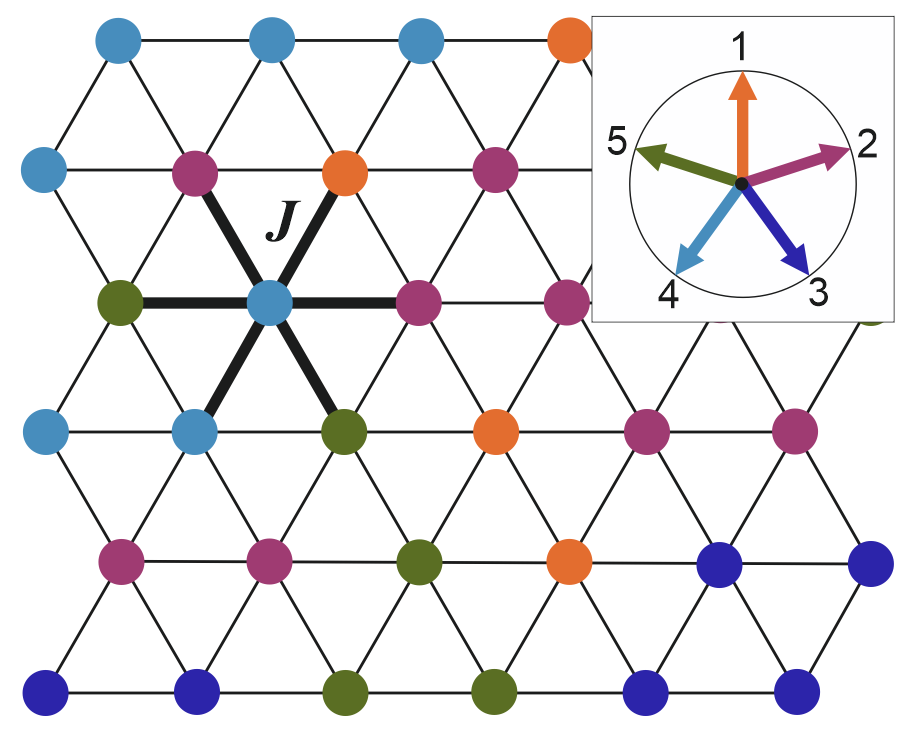
\includegraphics[width=0.8\textwidth]{mma/image2.png}
    \caption{Векторная модель Поттса с числом состояний спина $q = 5$ на треугольной решетке.}
    \label{fig:mma-1}
\end{figure}

\section{Метод исследований}

Исследования проводились на основе алгоритма Ванга-Ландау метода Монте-Карло (МК) \cite{bib:mma-9,bib:mma-10,bib:mma-11}. Данный алгоритм является реализацией метода энтропийного моделирования и его основной особенностью является возможность расчета функции плотности состояний системы, зная которую можно легко вычислить любые интересующие нас термодинамические параметры системы.

Алгоритм Ванга-Ландау является разновидностью энтропийного моделирования и, как показывает опыт его применения в последние годы, является весьма эффективным для исследования различных дискретных спиновых систем \cite{bib:mma-9}.

Алгоритм Ванга-Ландау основан на том, что совершая случайное блуждание в пространстве энергий с вероятностями, обратно пропорциональными плотности состояний $g(E)$, мы получаем равномерное распределение по энергиям. Подобрав вероятности перехода такими, что посещение всех энергетических состояний стало бы равномерным, можно получить изначально неизвестную плотность состояний $g(E)$, зная которую можно вычислить значения необходимых термодинамических параметров при любой температуре. Так как плотность состояний $g(E)$ очень быстро растет с увеличением размеров исследуемых систем, для удобства хранения и обработки больших чисел пользуются величиной $\ln g(E)$.

Важным обстоятельством является то, что плотность состояний $g(E)$ не зависит от температуры, следовательно, рассчитав ее однократно, мы можем вычислить значения любых термодинамических параметров системы при любой ненулевой температуре.

В данной работе нами алгоритм Ванга-Ландау был использован в следующем виде \cite{bib:mma-9,bib:mma-10,bib:mma-11}:
\begin{itemize}
    \item Задается произвольная начальная конфигурация спинов. Стартовые значения плотности состояний $g(E)=1$, гистограммы распределений по энергиям $H(E)=1$ и начальное значение модификационного фактора $f = f_0 = e^1 \approx 2.71828$.
    \item Многократно совершаем шаги в фазовом пространстве, пока не получим относительно плоскую гистограмму $H(E)$ (т.е. пока не будут посещены примерно одинаковое количество раз все возможные энергетические состояния системы). В качестве критерия <<плоскости>> гистограммы нами принималось условие отклонения числа посещений всех возможных (с ненулевой плотностью $g(E) \neq 1$) энергетических состояний на величину не более чем на 10\% от среднего значения по системе.
    \item При этом вероятность перехода из состояния с энергией $E_1$ в состояние с энергией $E_2$ определяется по формуле $p = g(E_1) / g(E_2)$. Если переход в состояние с энергией $E_2$ состоялся, то для энергии $E_2$ проводится модификация плотности состояния $g(E_2) \to f \times g(E_2)$, и гистограммы $H(E_2) \to H(E_2) + 1$ иначе меняем параметры для энергии $E_1$ $g(E_1) \to f \times g(E_1)$ $H(E_1) \to H(E_1) + 1$.
    \item Если гистограмма стала <<плоской>>" то: обнуляем гистограмму $H(E) \to 0$,  уменьшаем модификационный фактор $f \to \sqrt{f}$, и продолжаем снова и снова, пока модификационный фактор $f \geq f_{\min}$. В качестве минимального значения модификационного фактора нами принималось $f_{\min} = 1.0000000001$.
    \item Каждый раз при достижении энергетического минимума нами проводился анализ магнитной структуры основного состояния и его запись в графический файл. При этом проводилось сравнение полученной конфигурации с ранее полученными и только при обнаружении новой уникальной конфигурации производится ее сохранение в графический файл. Далее данная структура заносится в специальную базу данных для данной модели для дальнейшего сравнения. Данная процедура позволяет избежать дублирования в графических файлах многократно встречающихся состояний с одинаковой магнитной структурой.
    \item После расчета плотности состояний системы для любой интересующей нас температуры рассчитываются различные термодинамические параметры, такие как, энтропия, внутренняя энергия, свободная энергия, теплоемкость, намагниченность, восприимчивость и т.д.
\end{itemize}

Более подробно алгоритм Ванга-Ландау изложен в работах \cite{bib:mma-9,bib:mma-10,bib:mma-11}.

\section{Векторная пятихвершинная модель Поттса на треугольной решетке}

На рис.~\ref{fig:mma-2} приведены плотности состояний $g(E)$ для разных линейных размеров системы для ферромагнитной и антиферромагнитной моделей (здесь и далее статистическая погрешность не превышает размеров символов, использованных для построения зависимостей). Как видно на рисунке, плотность состояний имеет куполообразную форму. С увеличением линейных размеров системы максимум плотности состояний $g(E)$ значительно возрастает.
\begin{figure}[ht]
    \begin{subfigure}{0.5\textwidth}
        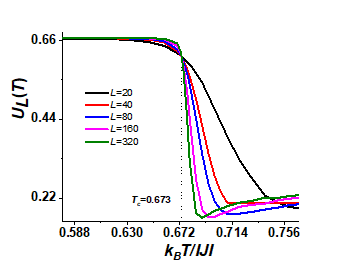
\includegraphics[width=0.9\linewidth]{mma/image17.png}
        \caption{для ферромагнитной модели;}
    \end{subfigure}
    \begin{subfigure}{0.5\textwidth}
        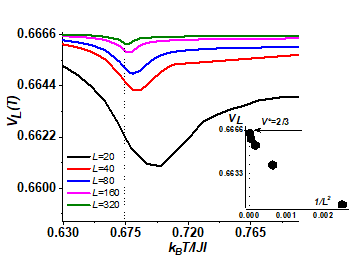
\includegraphics[width=0.9\linewidth]{mma/image18.png}
        \caption{для антиферромагнитной модели;}
    \end{subfigure}
    \caption{Плотность состояний $g(E)$ при различных линейных размерах $L$.}
    \label{fig:mma-2}
\end{figure}

На рис.~\ref{fig:mma-3}. представлены характерные зависимости теплоемкости $C$ от температуры для ферромагнитной и антиферромагнитной моделей с различными линейными размерами системы $L$. Отметим, что для ферромагнитной модели (рис.~\ref{fig:mma-3a}) на зависимостях теплоемкости $C$ от температуры для всех систем вблизи критической температуры наблюдаются два хорошо выраженных максимума. Наличие двух максимумов на температурной зависимости теплоемкости позволяет говорить о двух последовательных ФП в данной модели.
\begin{figure}[ht]
    \begin{subfigure}{0.5\textwidth}
        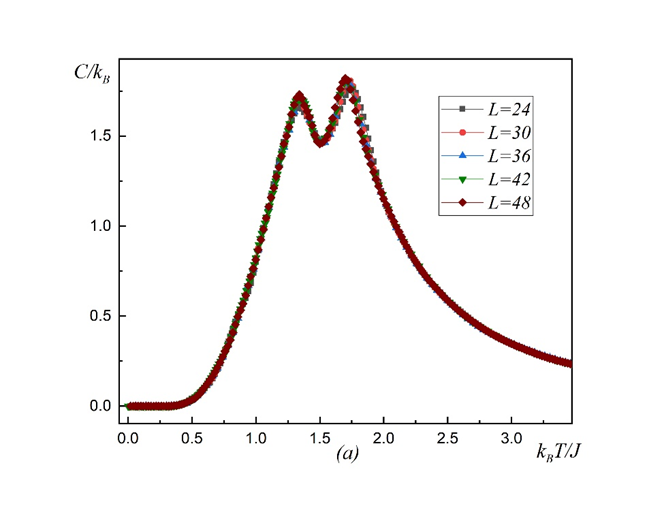
\includegraphics[width=0.9\linewidth]{mma/image19.png}
        \caption{для ферромагнитной модели;}
        \label{fig:mma-3a}
    \end{subfigure}
    \begin{subfigure}{0.5\textwidth}
        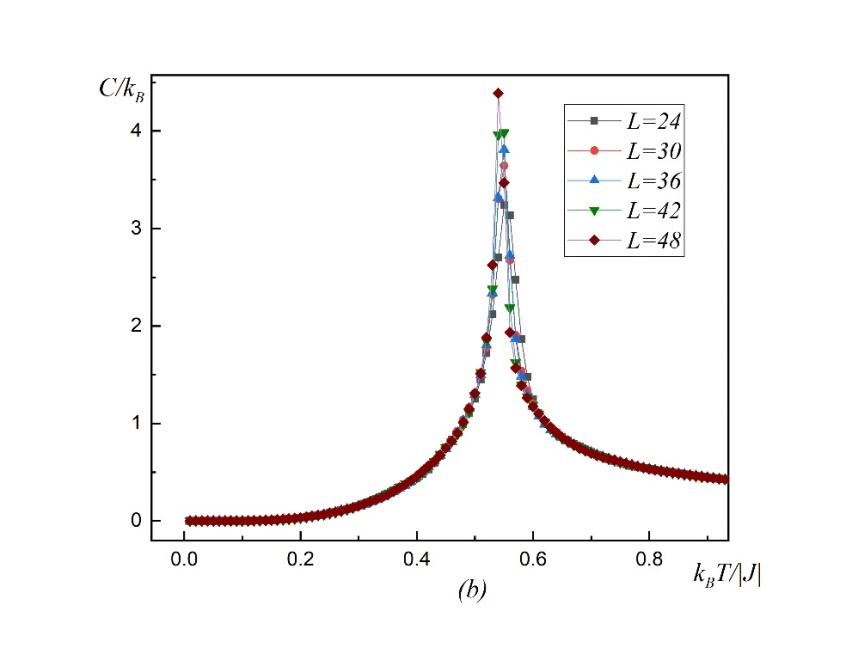
\includegraphics[width=0.9\linewidth]{mma/image20.jpeg}
        \caption{для антиферромагнитной модели;}
        \label{fig:mma-3b}
    \end{subfigure}
    \caption{Зависимость теплоемкости $C/k_B$ от температуры $k_B T/ \left|J\right|$ для разных $L$.}
    \label{fig:mma-3}
\end{figure}

\begin{figure}[ht]
    \begin{subfigure}{0.33\textwidth}
        
\includegraphics[width=0.9\linewidth]{mma/image21.png}
        \caption{в интервале температур $0 \leq T < Tc_1$;}
        \label{fig:mma-4a}
    \end{subfigure}
    \begin{subfigure}{0.33\textwidth}
        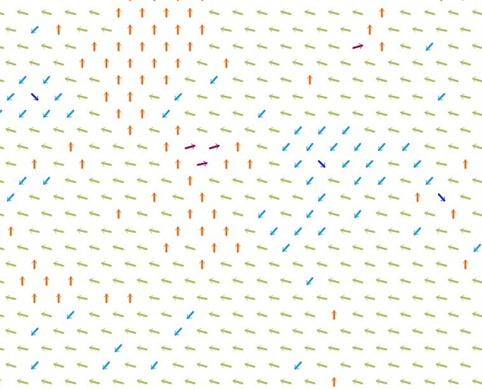
\includegraphics[width=0.9\linewidth]{mma/image22.png}
        \caption{в интервале температур $Tc_1 < T < Tc_2$;}
        \label{fig:mma-4b}
    \end{subfigure}
    \begin{subfigure}{0.33\textwidth}
        
\includegraphics[width=0.9\linewidth]{mma/image23.png}
        \caption{$T > Tc_2$;}
        \label{fig:mma-4c}
    \end{subfigure}
    \caption{Магнитные структуры основного состояния для ферромагнитной модели;}
    \label{fig:mma-4}
\end{figure}

Для антиферромагнитной модели (рис.~\ref{fig:mma-3b}) наблюдается только один максимум, что позволяет говорить об одном ФП. Все максимумы увеличиваются с ростом числа спинов в системе, причем они в пределах погрешности приходятся на одну и ту же температуру даже для систем с наименьшим значением $L$. Это свидетельствует, во-первых, о высокой эффективности использованного способа добавления периодических граничных условий, а во-вторых, о достижении насыщения по $N$ для многих исследуемых нами параметров.

Для определения типа упорядочения нами проведен анализ магнитных структур основного состояния в широком температурном интервале. На рис.~\ref{fig:mma-4} приведены полученные нами структуры. На рисунке видно, что в данной модели наблюдаются три типа магнитного упорядочения: в интервале температур $0 \leq T < Tc_1$ (рис.~\ref{fig:mma-4a}) наблюдается полностью упорядоченная ферромагнитная фаза; в интервале $Tc_1 < T < Tc_2$ (рис.~\ref{fig:mma-4b}) -- фаза типа Березинского-Костерлица-Таулеса, где наблюдается ближний порядок в системе, в котором превалирует одно из пяти состояний спина; при дальнейшем повышении температуры $T > Tc2$ (рис.~\ref{fig:mma-4c}) -- полностью разупорядоченная парамагнитная фаза.

\begin{figure}[ht]
    \begin{subfigure}{0.5\textwidth}
        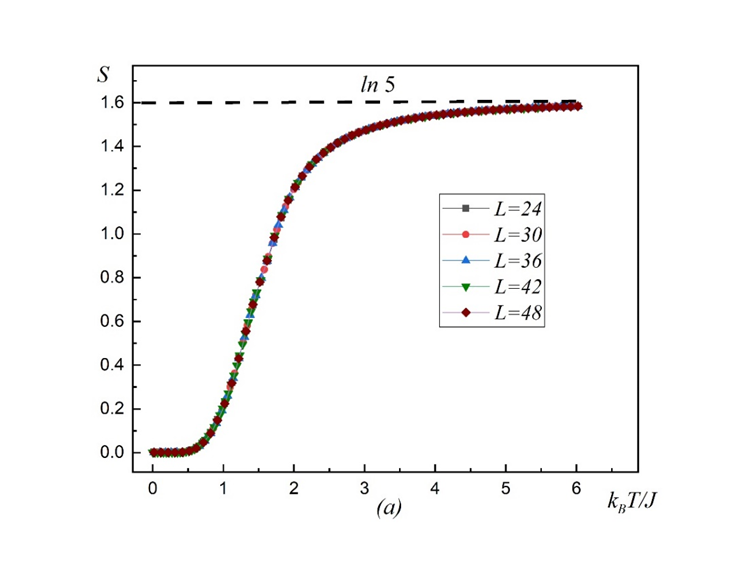
\includegraphics[width=0.9\linewidth]{mma/image24.png}
        \caption{для ферромагнитной модели;}
    \end{subfigure}
    \begin{subfigure}{0.5\textwidth}
        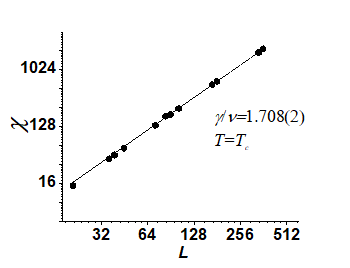
\includegraphics[width=0.9\linewidth]{mma/image25.png}
        \caption{для антиферромагнитной модели;}
    \end{subfigure}
    \caption{Температурные зависимости энтропии $S$.}
    \label{fig:mma-5}
\end{figure}

На рис.~\ref{fig:mma-5} приведены температурные зависимости энтропии $S$ для обоих моделей. Из рисунков видно, что с увеличением температуры энтропия для всех систем стремится к теоретически предсказанному значению $\ln 5$. При низких температурах, близких к абсолютному нулю, для ферромагнитной модели энтропия стремится к нулевому значению для всех значений $L$. Нулевая остаточная энтропия свидетельствует об отсутствии вырождения основного состояния. Для антиферромагнитной модели энтропия при низких температурах стремится к ненулевому значению для всех значений $L$. Такое поведение свидетельствует о сильном вырождении данной модели, что также характерно для фрустрированных систем.

Для анализа характера ФП использовался метод кумулянтов Биндера четвертого порядка по энергии, который имеет следующий вид:
\begin{equation}
    \label{eq:mma-2}
    V_L (T) = 1 - \frac{\left<E^4\right>}{\left<E^2\right>^2}
\end{equation}

Известно, что ФП второго рода характеризуются следующими отличительными особенностями: усредненная величина $V_L (T)$ стремится к тривиальному значению согласно выражению $V_L (T) = V* + b L^{-d}$ при $L \to \infty$ и $T = T(L)$, где $V* = 2/3$.

Характерные зависимости кумулянтов Биндера $V_L(T)$ от температуры для систем с линейными размерами для ферромагнтной и антиферромагнитной моделей приведены на рис.~\ref{fig:mma-6}. Как видим из рисунков энергетические кумулянты для обоих моделей показывают разный характер поведения. Для антиферромагнитного случая на графиках зависимости энергетических кумулянтов наблюдаются минимумы в области температуры фазового перехода, которые уменьшаются с увеличением размеров системы $L$. Для ферромагнитной модели такие минимумы не наблюдаются. Заметим, что на вставке к рис.~\ref{fig:mma-6b} наглядно видно, что тривиальная величина $V* \to 2/3$ при $L \to \infty$. Такое поведение, как отмечалось выше, характерно для ФП второго рода.
\begin{figure}[ht]
    \begin{subfigure}{0.5\textwidth}
        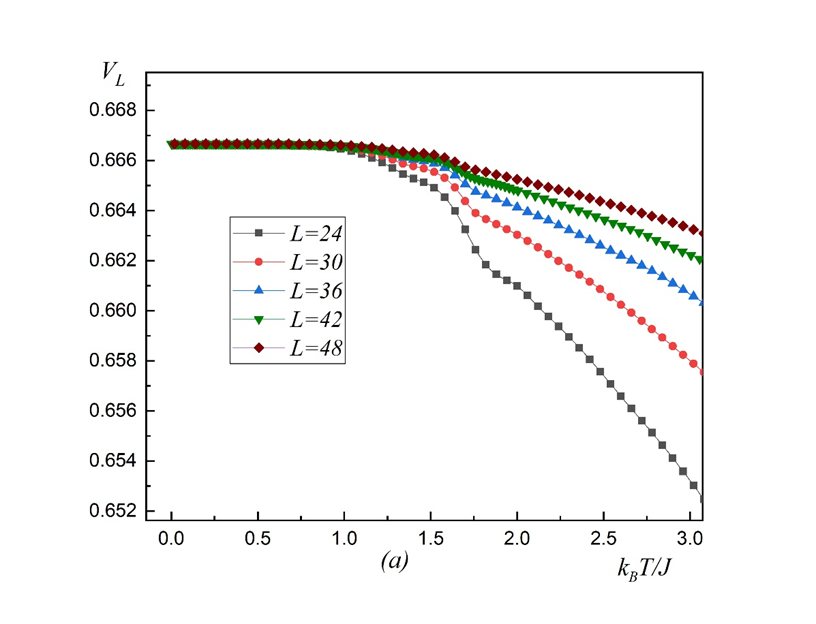
\includegraphics[width=0.9\linewidth]{mma/image27.png}
        \caption{для ферромагнитной модели;}
        \label{fig:mma-6a}
    \end{subfigure}
    \begin{subfigure}{0.5\textwidth}
        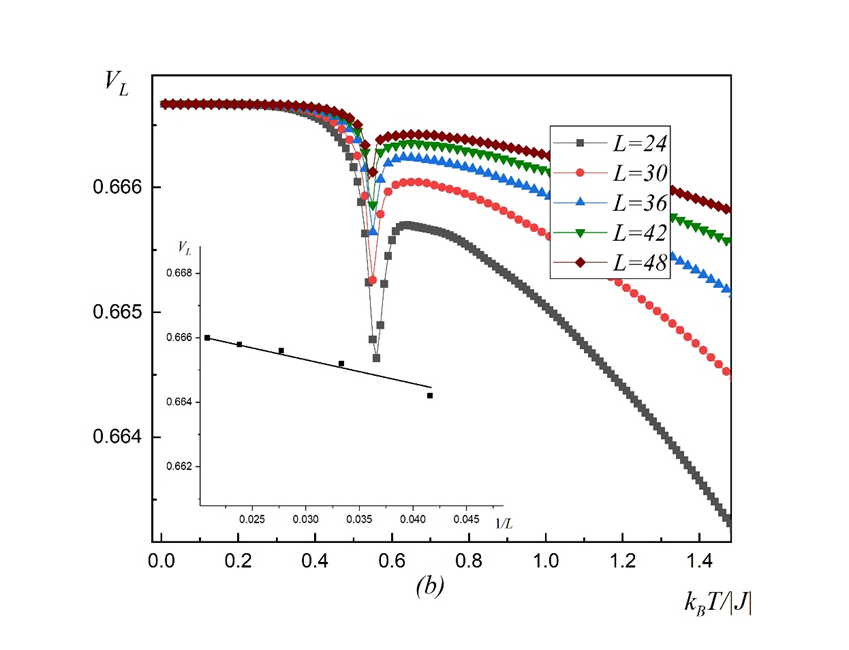
\includegraphics[width=0.9\linewidth]{mma/image28.png}
        \caption{для антиферромагнитной модели;}
        \label{fig:mma-6b}
    \end{subfigure}
    \caption{Температурная зависимость кумулянтов Биндера $V_L (T)$.}
    \label{fig:mma-6}
\end{figure}

Для более точного определения рода ФП мы использовали гистограммный анализ данных метода МК. В случае ФП первого рода на гистограмме распределения энергии вблизи температуры перехода наблюдается бимодальное распределение энергии. То есть, на графике появляются два максимума, расположенных симметрично относительно равновесного значения энергии. В случае ФП второго рода должен наблюдаться один максимум.

\begin{figure}[ht]
    \begin{subfigure}{0.5\textwidth}
        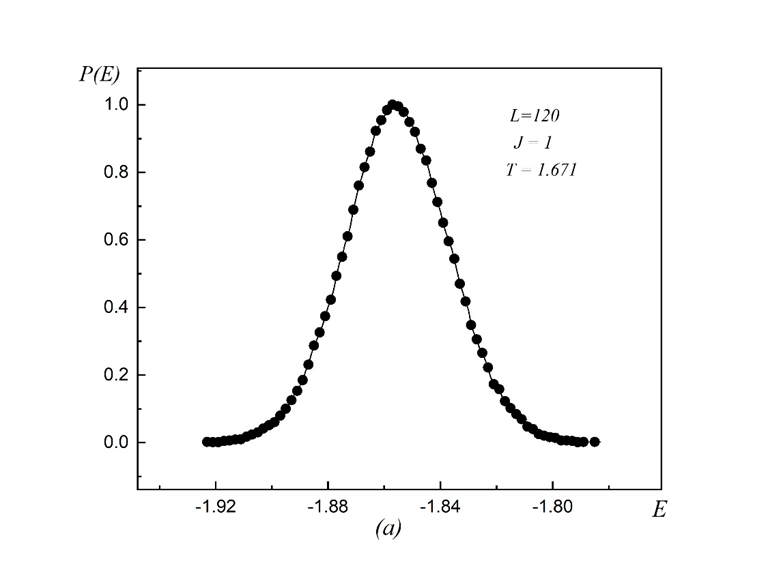
\includegraphics[width=0.9\linewidth]{mma/image29.png}
        \caption{для ферромагнитной модели;}
        \label{fig:mma-7a}
    \end{subfigure}
    \begin{subfigure}{0.5\textwidth}
        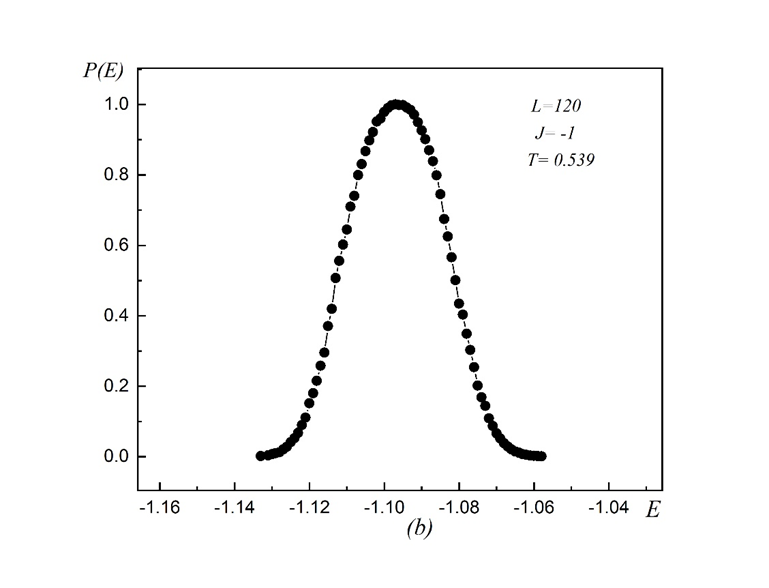
\includegraphics[width=0.9\linewidth]{mma/image30.png}
        \caption{для антиферромагнитной модели;}
        \label{fig:mma-7b}
    \end{subfigure}
    \caption{Гистограмма распределения энергии.}
    \label{fig:mma-7}
\end{figure}

На рис.~\ref{fig:mma-7a} и \ref{fig:mma-7b} представлены гистограммы распределения энергии для линейных размеров системы $L =120$ в области температуры ФП для ферромагнитной и антиферромагнитной моделей. На графиках зависимости вероятности $P$ от энергии системы $E$ наблюдается один хорошо выраженный максимум, который свидетельствует о наличии в антиферромагнитной модели ФП второго рода. Для ферромагнитной часовой модели подобный анализ показывает наличие одного максимума, который позволяет нам утверждать, что в данной модели точно не наблюдается ФП первого рода. Такое поведение характерно для ФП второго рода. Однако, анализ магнитных структур основного состояния свидетельствует в пользу перехода типа Березинского-Костерлица-Таулеса (рис.~\ref{fig:mma-4}).

%\section*{Заключение}
%
%Выполнено исследование магнитных структур основного состояния, фазовых переходов и термодинамических свойств двумерной векторной модели Поттса с числом состояний спина $q=5$ на треугольной решетке. В работе использован алгоритм Ванга-Ландау энтропийного метода Монте-Карло. Получены магнитные структуры основного состояния. Анализ полученных данных показывает, что для ферромагнитной модели на температурной зависимости теплоемкости наблюдаются два максимума. На основе метода кумулянтов Биндера и гистограммного метода проведен анализ рода ФП данной модели. Обнаружено, что для ферромагнитной модели происходят два фазовых перехода типа Березинского-Костерлица-Таулеса. Данные полученные для антиферромагнитной часовой модели свидетельствуют о том, что основное состояние системы сильно вырождено и в системе происходит ФП второго рода. Показано, что антиферромагнитное обменное взаимодействие ближайших соседей может повлиять на физические свойства векторной модели Поттса с числом состояний $q=5$.
%
%Таким образом, по проделанной работе можно сделать следующие выводы:
%\begin{itemize}
%    \item Предложена векторная модель Поттса с числом состояний $q=5$ на треугольной решетке;
%    \item Разработана программа для ЭВМ, основанная на новейшем алгоритме Ванга-Ландау, позволяющая исследовать векторную модель Поттса с числом состояний $q=5$ на треугольной решетке;
%    \item Методом Ванга-Ландау вычислены плотности состояний $g(E)$ для векторной модели Поттса с числом состояний $q=5$ на треугольной решетке.
%    \item Определены магнитные структуры основного состояния;
%    \item Рассчитаны температурные зависимости различных термодинамических параметров, таких как свободная энергия $F$, внутренняя энергия $E$, энтропия $S$, теплоемкость  $C$;
%    \item Показано, что энтропия для данной модели при температурах близких к абсолютному нулю для ферромагнитного случая стремится к нулю, а для антиферромагнитного случая стремится к $S_0=0.333$, которое соответствует сильно вырожденному состоянию. С повышением температуры энтропия во всех случаях стремится к теоретически предсказанному значению $\ln 5$;
%\end{itemize}
%
%Результаты, полученные в ходе исследований, могут быть полезными для описания различных низкоразмерных магнитных материалов, имеющих треугольную структуру.

%\section*{Публикации}
%
%\begin{enumerate}
%    \item Муртазаев А.К., Бадиев М.К., Магомедов М.А., Рамазанов М.К. Термодинамическое поведение двумерной часовой модели с числом состояний спина q = 5 // ФТТ. 2023. Т.65. вып. 8. С. 1399 -- 1402.  DOI: 10.21883/FTT.2023.08.56161.78.
%    \item Бабаев А.Б., Муртазаев А.К. Моделирование трехкомпонентной модели Поттса на гексагональной решетке методом Монте-Карло // Физика металлов и металловедение. 2023. Т.124. № 7. С. 577--583. Babaev A.B., Murtazaev A.K. Simulation of the three-component Potts model on a hexagonal lattice by the Monte Carlo method // Physics of Metals and Metallography, vol. 124, No. 7, pp. 221--225 (2023) Published: 26 May 2023 DOI:10.31857/S0015323023600454
%\end{enumerate}
%
%\textbf{Публикации в трудах международных и российских конференций:}
%\begin{enumerate}
%    \item Бадиев М.К., Муртазаев А.К., Магомедов М.А., Рамазанов М.К. Критическое поведение часовой модели с числом состояний спина q = 5 на треугольной решетке // Сборник трудов международной конференции «Фазовые переходы, критические и нелинейные явления в конденсированных средах». Махачкала, 10-15 сентября 2023г., С.50-52. \url{https://www.dagphys.ru/upload/files/conference/2023_Conference.pdf}
%\end{enumerate} 